\documentclass[11pt,a4paper]{article}
\usepackage[utf8]{inputenc}
\usepackage[T1]{fontenc}
\usepackage[spanish,es-nodecimaldot]{babel}
\usepackage[margin=2.5cm]{geometry}
\usepackage{graphicx}
\usepackage{booktabs}
\usepackage{tabularx}
\usepackage{array}
\usepackage{float}
\usepackage{xcolor}
\usepackage{tikz}
\usetikzlibrary{arrows.meta,positioning,calc,fit}
\usepackage{csquotes}
\usepackage[backend=biber,style=ieee]{biblatex}
\addbibresource{referencias.bib}
\usepackage[hidelinks]{hyperref}

\title{Análisis crítico de un sistema distribuido: HDFS comparado con Ceph}
\author{Silva Triviño John Jairo}
\date{13 de noviembre de 2026}

\begin{document}

% ------------------------------------------------------------------ PORTADA
\begin{titlepage}
\centering
{\large Universidad Técnica Estatal de Quevedo\par}
\vspace{0.4cm}
{\large Facultad de Ciencias de la Computación\par}
\vspace{0.4cm}
{\large Carrera: Software\par}
\vspace{1.5cm}
{\LARGE\bfseries Análisis crítico de un sistema distribuido:\\ HDFS comparado con Ceph\par}
\vspace{1.5cm}
{\large Informe académico individual (Unidad 1)\par}
\vspace{1.5cm}
\begin{tabular}{@{}ll@{}}
\textbf{Asignatura:} & Sistemas Distribuidos\\[4pt]
\textbf{Código de la actividad:} & TA-IND-01\\[4pt]
\textbf{Estudiante:} & Silva Triviño John Jairo\\[4pt]
\textbf{Semestre y paralelo:} & Séptimo semestre, paralelo A\\[4pt]
\textbf{Docente:} & Guerrero Ulloa Gleiston Cicerón\\[4pt]
\textbf{Grupo:} & TA-GHLZ\\[4pt]
\textbf{Fecha:} & 13 de noviembre de 2026
\end{tabular}\par
\vspace{0.8cm}
\textbf{Repositorio:}\par\smallskip
{\small\url{https://github.com/ameraj2-bit/ta-ind-01-sistemas-distribuidos}\par}
\vfill
\end{titlepage}

% ------------------------------------------------------------------ RESUMEN
\begin{abstract}
Este informe analiza el Hadoop Distributed File System (HDFS) como sistema distribuido real y lo compara con Ceph. Describo su arquitectura, con un NameNode que guarda los metadatos y varios DataNodes que guardan bloques replicados, y evalúo qué transparencias ofrece, cómo se ubica frente a los teoremas CAP y PACELC, qué modelos de comunicación usa y cómo tolera fallos, incluido un incidente real documentado en LinkedIn. Para comprobarlo monté un clúster propio con Docker, de un NameNode y cuatro DataNodes, y apagué uno mientras leía un archivo de 300 MB. El NameNode tardó 14 min 02 s en declarar muerto al nodo; aun así el archivo siguió disponible y sus bloques volvieron a tener tres réplicas. Contrasto estos resultados con dos situaciones de mi entorno, el SGA de la UTEQ y WhatsApp, y con Ceph, que ubica los datos mediante el algoritmo CRUSH y no mediante un servidor central. Concluyo que HDFS es adecuado para archivos grandes que se escriben una vez, pero que su NameNode único concentra el riesgo y limita el crecimiento.
\end{abstract}

\newpage
% ------------------------------------------------------------------ 1. INTRODUCCION
\section{Introducción}
Un sistema distribuido reparte datos y trabajo entre varias máquinas que se coordinan mediante mensajes, y debe seguir funcionando aunque alguna falle. Elegí HDFS porque es un caso claro de ese problema: guarda archivos muy grandes dividiéndolos en bloques que se copian en distintas máquinas. Como segundo sistema para comparar elegí Ceph, que resuelve el mismo problema de otra forma: en lugar de un servidor que recuerda dónde está cada dato, calcula la ubicación \cite{CephArchitecture}.

El objetivo es entender y evaluar de forma crítica cómo HDFS responde a las propiedades de la Unidad 1: transparencia, consistencia y disponibilidad, comunicación y tolerancia a fallos. El trabajo combina tres fuentes de evidencia: documentación y artículos citados, un experimento propio de caída de un DataNode y situaciones reales de mi entorno. El informe sigue este orden: arquitectura (sección~\ref{sec:arq}), análisis (sección~\ref{sec:analisis}), experimento (sección~\ref{sec:exp}), ejemplos del entorno (sección~\ref{sec:ejemplos}), comparación con Ceph (sección~\ref{sec:comp}), postura crítica y conclusiones.

% ------------------------------------------------------------------ 2. ARQUITECTURA
\section{Arquitectura de HDFS}\label{sec:arq}
HDFS sigue un esquema maestro y trabajadores. El \textbf{NameNode} es el árbitro y el repositorio de todos los metadatos de HDFS \cite{HadoopHDFSDesign}: el árbol de directorios y, para cada archivo, la lista de bloques y los DataNodes donde está cada uno. Los \textbf{DataNodes} guardan los bloques; un tamaño típico de bloque es de 128 MB \cite{HadoopHDFSDesign}. Cada DataNode envía periódicamente un latido (\emph{heartbeat}) al NameNode, y el NameNode detecta un problema por la ausencia de ese latido \cite{HadoopHDFSDesign}. Los archivos son de escritura única (salvo anexos y truncados) y tienen un solo escritor a la vez \cite{HadoopHDFSDesign}.

La figura~\ref{fig:arq} muestra el clúster que armé para el experimento. Los tres bloques del archivo de prueba aparecen con la ubicación real que devolvió el comando \texttt{hdfs fsck} (sección~\ref{sec:exp}).

\begin{figure}[H]
\centering
\begin{tikzpicture}[
  box/.style={draw, rounded corners=2pt, minimum height=0.9cm, align=center, font=\small},
  nn/.style={box, minimum width=7.2cm, fill=blue!8},
  cl/.style={box, minimum width=2.2cm, fill=gray!12},
  dn/.style={box, minimum width=2.6cm, minimum height=1.9cm, fill=green!8, anchor=north},
  blk/.style={draw, fill=white, minimum width=0.6cm, minimum height=0.45cm, font=\scriptsize, inner sep=1pt},
  ctrl/.style={-{Latex[length=2mm]}, thick},
  data/.style={-{Latex[length=2mm]}, thick, blue!60!black},
  hb/.style={-{Latex[length=2mm]}, dashed, red!70!black}
]
\node[nn] (nn) at (0,0) {\textbf{NameNode}\\ metadatos: archivo $\to$ bloques $\to$ DataNodes};
\node[cl] (cl) at (-6.7,0) {Cliente\\ \texttt{hdfs dfs}};

\node[dn] (d1) at (-4.4,-3.6) {\textbf{DataNode 1}\\ 172.21.0.6};
\node[dn] (d2) at (-1.47,-3.6) {\textbf{DataNode 2}\\ 172.21.0.3};
\node[dn] (d3) at (1.47,-3.6)  {\textbf{DataNode 3}\\ 172.21.0.5};
\node[dn] (d4) at (4.4,-3.6)  {\textbf{DataNode 4}\\ 172.21.0.4};

% Bloques segun el fsck de las 23:24 (cada bloque con 3 replicas)
\node[blk] at ($(d1.south)+(0,0.35)$) {B0};
\node[blk] at ($(d2.south)+(-0.4,0.35)$) {B1};
\node[blk] at ($(d2.south)+(0.4,0.35)$) {B2};
\node[blk] at ($(d3.south)+(-0.8,0.35)$) {B0};
\node[blk] at ($(d3.south)+(0,0.35)$) {B1};
\node[blk] at ($(d3.south)+(0.8,0.35)$) {B2};
\node[blk] at ($(d4.south)+(-0.8,0.35)$) {B0};
\node[blk] at ($(d4.south)+(0,0.35)$) {B1};
\node[blk] at ($(d4.south)+(0.8,0.35)$) {B2};

\draw[ctrl] (cl) -- node[above, font=\scriptsize] {1. ¿dónde está?} (nn);
\draw[data] (cl.south) |- (d1.west);
\node[font=\scriptsize, blue!60!black, align=center, anchor=east] at (-6.8,-2.0) {2. lee o escribe\\ bloques directo\\ en los DataNodes};
\foreach \d in {d1,d2,d3,d4}{
  \draw[hb] (\d.north) -- (nn.south -| \d.north);
}
\node[font=\scriptsize, red!70!black, anchor=west] at (4.5,-1.0) {latidos};
\end{tikzpicture}
\caption{Clúster del experimento: 1 NameNode y 4 DataNodes, replicación 3. B0, B1 y B2 son los tres bloques de \texttt{/datos.bin} (300 MB); su ubicación proviene de mi \texttt{fsck} (captura-05). Línea discontinua: latidos. Línea azul: lectura o escritura directa de bloques (en la escritura los DataNodes se encadenan en una tubería). Diagrama propio dibujado en TikZ a partir de mi boceto a mano.}
\label{fig:arq}
\end{figure}

\subsection{Evolución desde mi boceto a mano}
Mi primer esquema (Anexo~A, fechado 12/11/2026) mostraba un NameNode, tres DataNodes y un cliente, con los pasos «1. ¿Dónde está el archivo?» y «2. Lee los bloques directo de un DataNode», los latidos cada pocos segundos, una tubería de escritura DN1 $\to$ DN2 $\to$ DN3 y los racks como elemento opcional. Los cambios al diagrama definitivo fueron:
\begin{itemize}
  \item \textbf{Cuatro DataNodes en lugar de tres.} Con tres nodos y factor de replicación 3, todos los bloques están en todos los nodos y, si uno cae, no queda un nodo libre donde recrear la réplica. Con cuatro hay un nodo disponible para ello.
  \item \textbf{Ubicación real de los bloques.} En el boceto cada DataNode tenía los bloques A y B. En el clúster real el archivo se dividió en tres bloques (128 MB, 128 MB y 44 MB) y la ubicación no es uniforme: el DataNode 1 solo tiene B0.
  \item \textbf{Datos reales del montaje:} direcciones IP, un solo rack, y el NameNode atendiendo solicitudes en el puerto 8020 y la interfaz web en el 9870.
\end{itemize}

% ------------------------------------------------------------------ 3. ANALISIS
\section{Análisis desde los conceptos de la Unidad 1}\label{sec:analisis}

\subsection{Transparencias de distribución}
\begin{itemize}
  \item \textbf{Ubicación:} el cliente pide \texttt{/datos.bin} por su ruta y no indica en qué DataNode está cada bloque; esa información la resuelve el NameNode. Lo comprobé al leer el archivo completo sin conocer la ubicación de los bloques.
  \item \textbf{Replicación:} el usuario ve un solo archivo; HDFS mantiene tres copias de cada bloque (factor 3 en mi configuración).
  \item \textbf{Fallos:} con \texttt{datanode4} apagado la lectura completa funcionó con el mismo comando y la misma ruta (sección~\ref{sec:exp}). Esta transparencia es parcial: el cliente no vio el fallo, pero el administrador sí ve nodos muertos en los informes.
  \item \textbf{Concurrencia:} es limitada por diseño. HDFS admite un solo escritor por archivo \cite{HadoopHDFSDesign}, de modo que dos clientes no pueden escribir a la vez el mismo archivo.
\end{itemize}

\subsection{CAP y PACELC}
El teorema CAP establece un compromiso entre consistencia, disponibilidad y tolerancia a particiones: un sistema solo puede conservar dos de las tres. PACELC lo extiende: si hay partición (P), se elige entre disponibilidad (A) y consistencia (C); si no la hay (E), se elige entre latencia (L) y consistencia (C) \cite{Ahmed2023}. El artículo agrupa los sistemas en PC/EC, PC/EL, PA/EC y PA/EL, y en su lista de la página 172 figuran HBase y BigTable como PC/EC; HDFS no aparece clasificado.

\textbf{Mi clasificación de HDFS (razonamiento propio, no una clasificación publicada):} lo ubico del lado de la consistencia. El NameNode es el árbitro único de los metadatos y el archivo tiene un solo escritor \cite{HadoopHDFSDesign}; en mi montaje, que no tiene NameNode de respaldo, una falla del NameNode dejaría sin servicio al espacio de nombres antes que permitir vistas distintas del sistema de archivos. No probé esa caída. Mi experimento fue una falla de un DataNode, no una partición de red, así que no sirve como evidencia de PACELC: solo muestra que los datos siguieron disponibles gracias a la replicación.

Para Ceph, el artículo de Peters y van der Ster señala que CephFS busca ofrecer garantías de consistencia equivalentes a las de un sistema de archivos local \cite{Peters2021}, y la documentación indica que los monitores usan el algoritmo Paxos y una mayoría para acordar el mapa del clúster \cite{CephArchitecture}. Esto es coherente con una orientación a consistencia, pero tampoco es una clasificación publicada.

\subsection{Modelos de comunicación}
HDFS combina tres formas de comunicación:
\begin{itemize}
  \item \textbf{Cliente--servidor con llamada a procedimiento remoto} entre el cliente y el NameNode para preguntar ubicaciones (en mi configuración, \texttt{namenode:8020}). Es síncrona: el cliente espera la respuesta.
  \item \textbf{Transferencia directa de datos} entre el cliente y los DataNodes (puerto 9866 en las ubicaciones que mostró \texttt{fsck}), sin pasar por el NameNode. Esto evita que el NameNode sea un cuello de botella para los datos. Un estudio sobre archivos pequeños en HDFS describe el mismo flujo de lectura: el cliente pide al NameNode los metadatos (bloques y ubicaciones) y luego contacta a los DataNodes \cite{Alange2023}.
  \item \textbf{Mensajes periódicos (latidos)} de los DataNodes al NameNode \cite{HadoopHDFSDesign}, de tipo asíncrono y unidireccional. Su ausencia es la señal de falla.
\end{itemize}
En la escritura, los DataNodes que guardan las réplicas se encadenan en una tubería \cite{HadoopHDFSDesign}, como dibujé en mi boceto.

\subsection{Tolerancia a fallos}
Los mecanismos son tres: replicación de bloques, detección por latidos y re-replicación. Ante la ausencia de latidos, el NameNode lleva la cuenta de qué bloques necesitan replicarse e inicia la replicación cuando hace falta \cite{HadoopHDFSDesign}. Una revisión sobre tolerancia a fallos en sistemas de almacenamiento masivo describe el enfoque de latidos, usado en HDFS, YARN y Storm, y explica que un componente se declara fallido si no recibe el latido dentro de un tiempo especificado \cite{Saadoon2022}.

\textbf{Incidente real documentado.} En 2020 LinkedIn publicó el análisis de un incidente en su clúster Hadoop: por fallas de procedimiento en la gestión del ciclo de vida de los equipos, aproximadamente el 2\,\% de las máquinas de unos pocos racks fue reinstalado por error \cite{LinkedIn2020}. La pérdida fue pequeña en bloques (cerca del 0,02\,\%), pero el 10\,\% de sus flujos de trabajo falló porque basta un archivo corrupto para detener un flujo, y la recuperación tomó varios días \cite{LinkedIn2020}. Lo relevante para este informe es que la replicación no protege frente a errores que afecten a muchos nodos a la vez, y que la recuperación acelerada también estresa el sistema. En mi experimento fallaba un solo nodo, el caso para el que HDFS está diseñado.

\textbf{Límite del NameNode.} Un artículo sobre federación indica que HDFS escala los DataNodes pero no el NameNode, donde se gestionan los metadatos, lo que genera problemas de rendimiento y de crecimiento del espacio de nombres \cite{Dhulavvagol2023}.

% ------------------------------------------------------------------ 4. EXPERIMENTO
\section{Experimentación propia}\label{sec:exp}
\textbf{Montaje.} \texttt{docker compose} con la imagen \texttt{apache/hadoop:3}: 1 NameNode y 4 DataNodes, factor de replicación 3. Los archivos \texttt{docker-compose.yml} y \texttt{config}, junto con todos los comandos y salidas, están en la carpeta \texttt{experimento/} del repositorio. Subí un archivo de 300 MB (\texttt{/datos.bin}), que HDFS dividió en 3 bloques, cada uno con 3 réplicas.

\textbf{Procedimiento.} Apagué \texttt{datanode4} con \texttt{docker stop} a las 23:28:51 del 12/11/2026 y monitoreé el estado cada 60 s. Luego leí el archivo completo, revisé la ubicación de los bloques con \texttt{fsck} y volví a encender el nodo.

\begin{table}[H]
\centering\small
\begin{tabularx}{\textwidth}{@{}l>{\raggedright\arraybackslash}X@{}}
\toprule
Hora local & Observación \\
\midrule
23:24:35 & \texttt{fsck}: 3 bloques, cada uno con 3 réplicas, 4 DataNodes (captura-05) \\
23:28:51 & \texttt{docker stop datanode4} \\
23:31:12 & El NameNode aún muestra 4 DataNodes vivos \\
23:42:53 & Log del NameNode: \emph{lost heartbeat from 172.21.0.4} (captura-10) \\
23:52:47 & 1 DataNode muerto, 3 vivos, 0 bloques subreplicados (captura-08) \\
00:03:15 & \texttt{fsck}: 3 DataNodes, bloques con 3 réplicas, sin 172.21.0.4 (captura-09) \\
00:04:21 & Lectura completa con el nodo caído: 1,853~s (captura-09) \\
00:10:42 & \texttt{docker start datanode4} \\
00:11:10 & 4 DataNodes vivos, 0 bloques subreplicados (captura-11) \\
\bottomrule
\end{tabularx}
\caption{Línea de tiempo del experimento (horas locales, UTC$-$5).}
\end{table}

\textbf{Resultados.}
\begin{itemize}
  \item \textbf{Detección:} el NameNode declaró muerto al nodo 14 min 02 s después de apagarlo (23:28:51 $\to$ 04:42:53 UTC en el log). La detección no es inmediata: la documentación habla de ausencia de latidos \cite{HadoopHDFSDesign} y la revisión de Saadoon et al. de un tiempo especificado \cite{Saadoon2022}. No verifiqué con \texttt{hdfs getconf} los valores de latido configurados en mi clúster, así que no puedo explicar con certeza por qué fueron 14 min 02 s y no otro valor.
  \item \textbf{Disponibilidad y transparencia:} la lectura completa con 3 DataNodes vivos funcionó sin cambiar el comando, en 1,853~s; con 4 DataNodes tardó 1,690, 1,901 y 2,107~s (promedio 1,899~s). La diferencia entre 3 y 4 nodos (0,046~s) es menor que la variación entre lecturas con 4 nodos (0,417~s), así que no permite concluir nada sobre rendimiento.
  \item \textbf{Re-replicación:} antes de la falla el \texttt{datanode4} tenía una copia de cada bloque; a las 00:03:15 los bloques 1 y 2 estaban en los tres nodos restantes (172.21.0.3, .5 y .6) y el resumen de \texttt{fsck} indicaba replicación promedio 3,0 y 0 bloques subreplicados. No observé el proceso de copia, solo su resultado.
\end{itemize}

\begin{figure}[H]
\centering
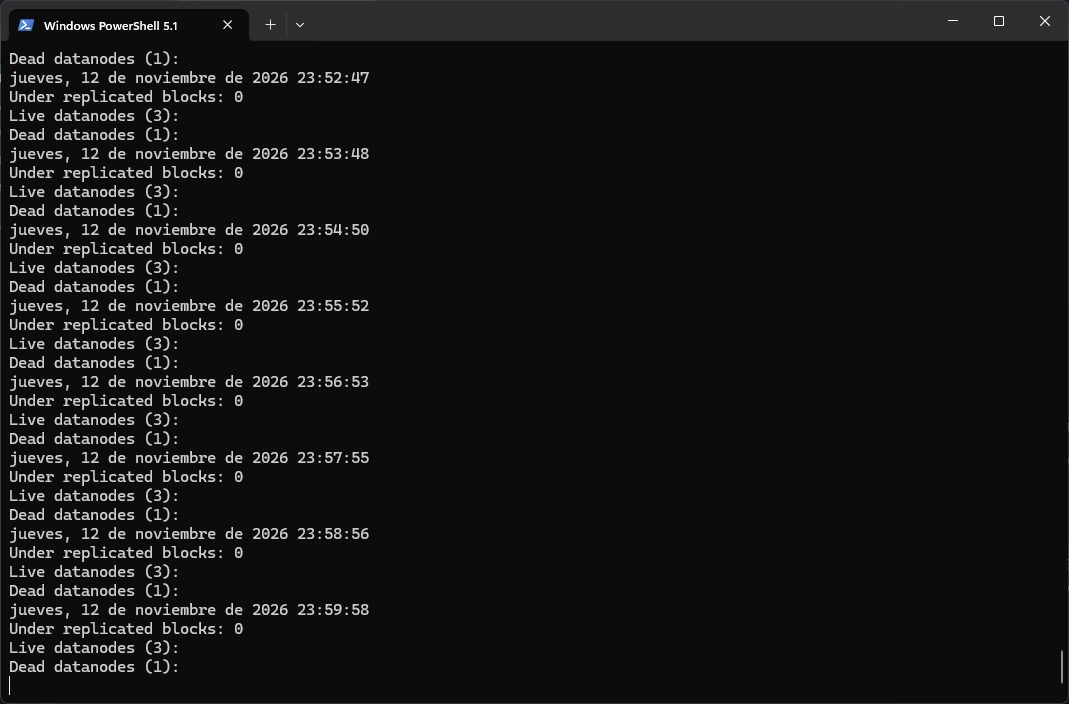
\includegraphics[width=0.92\textwidth]{../experimento/capturas/captura-08-dead-datanode.jpeg}
\caption{Captura propia (23:52): \texttt{Dead datanodes (1)}, \texttt{Live datanodes (3)} y 0 bloques subreplicados.}
\end{figure}

\begin{figure}[H]
\centering
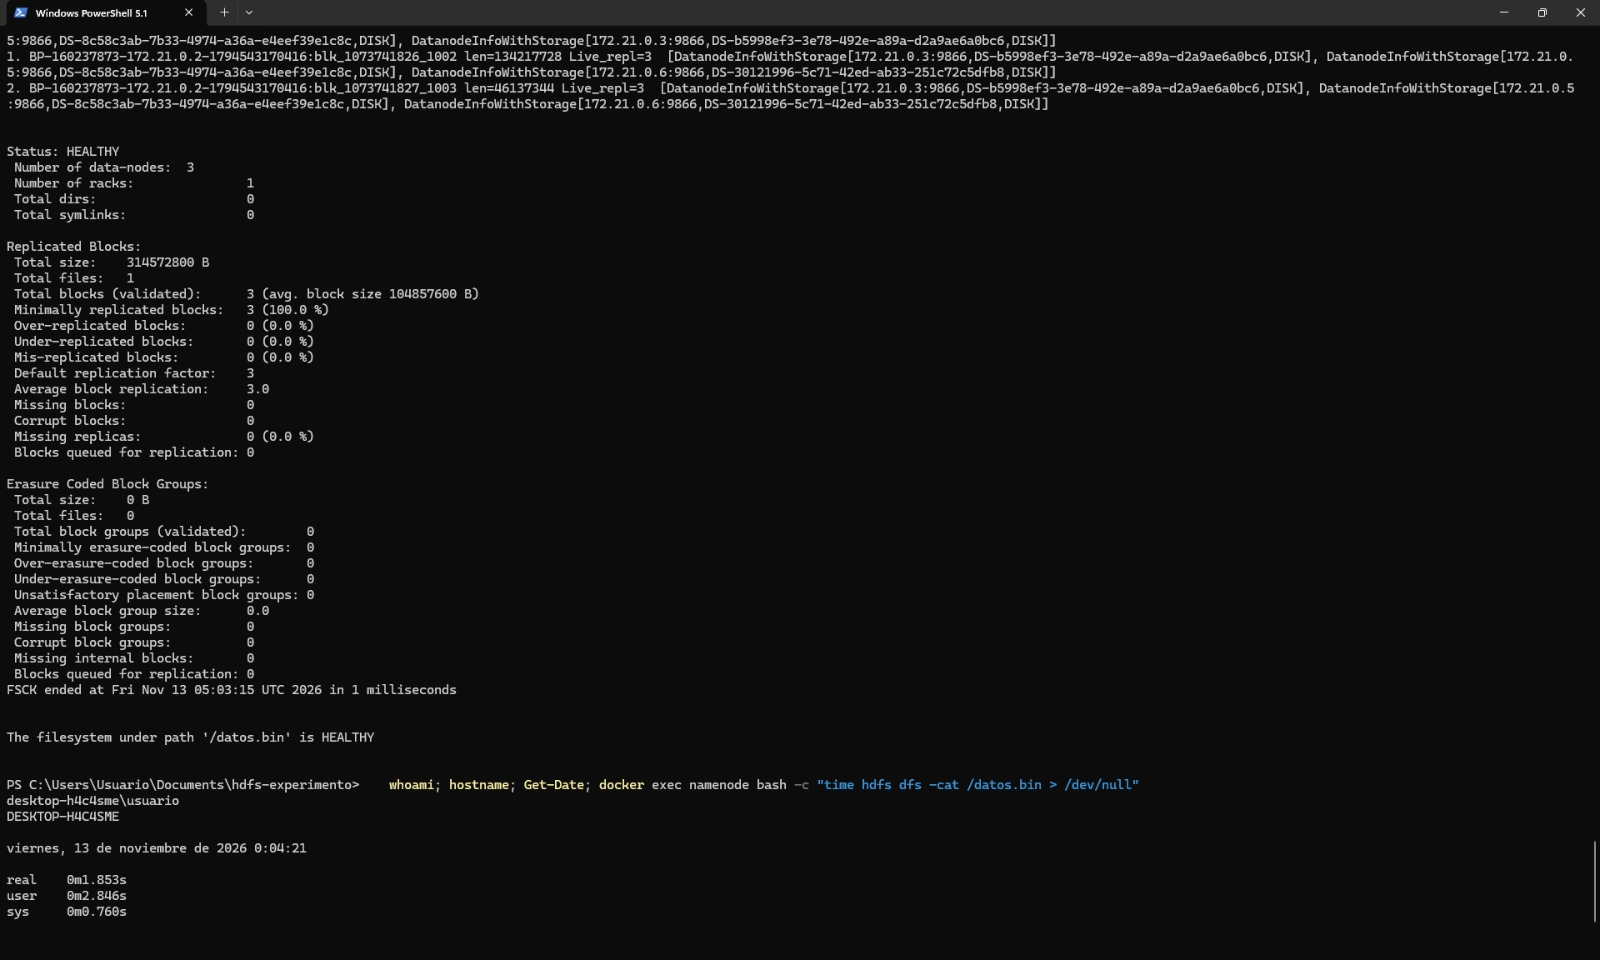
\includegraphics[width=0.92\textwidth]{../experimento/capturas/captura-09-lectura-nodo-caido.jpeg}
\caption{Captura propia (00:03--00:04): \texttt{fsck} con 3 DataNodes y lectura completa con el nodo caído.}
\end{figure}

\begin{figure}[H]
\centering
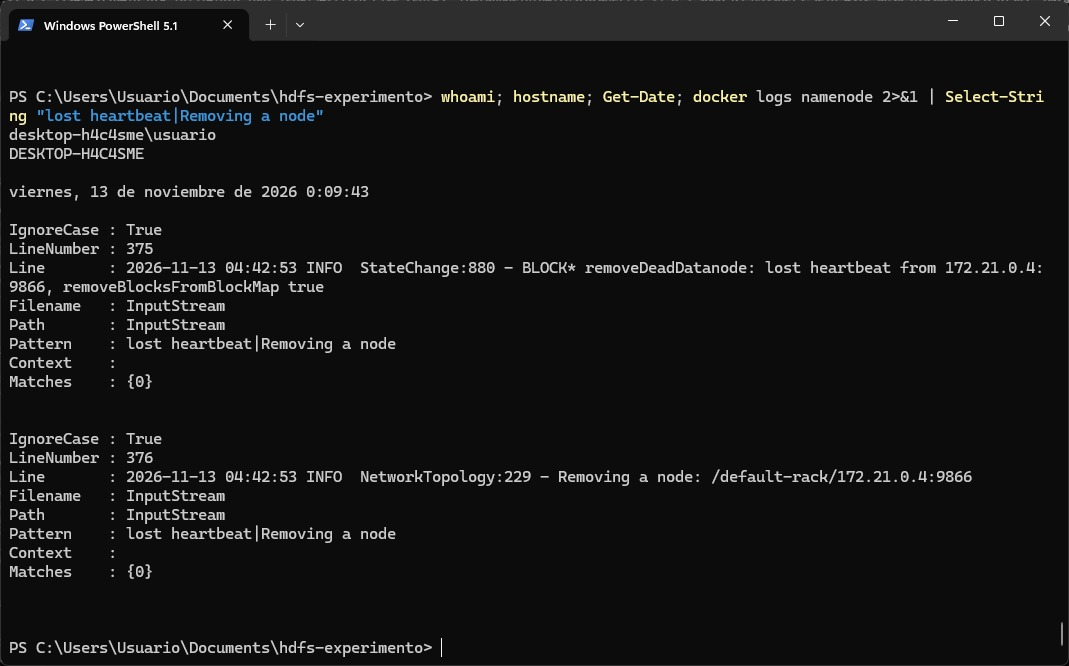
\includegraphics[width=0.92\textwidth]{../experimento/capturas/captura-10-log-nodo-muerto.jpeg}
\caption{Captura propia: mensaje del NameNode \emph{lost heartbeat from 172.21.0.4:9866}.}
\end{figure}

\begin{figure}[H]
\centering
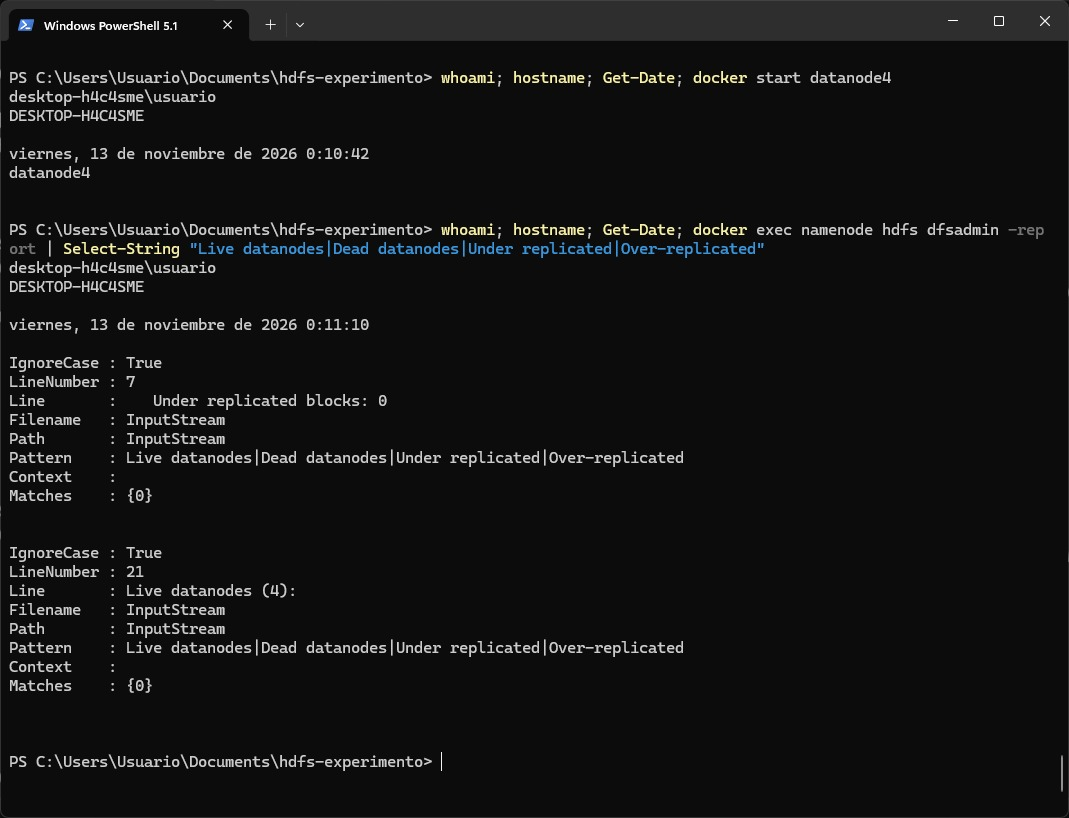
\includegraphics[width=0.92\textwidth]{../experimento/capturas/captura-11-nodo-recuperado.png.jpeg}
\caption{Captura propia (00:11): nodo recuperado, 4 DataNodes vivos y 0 bloques subreplicados.}
\end{figure}

\textbf{Limitaciones.} Los cuatro DataNodes comparten el disco de mi computador, así que simulé la caída de un contenedor y no una falla independiente de almacenamiento. Monitoreé cada 60 s, por lo que no capté el instante de la re-replicación. Hice una sola repetición y no medí la lectura antes de la falla ni durante los minutos en que el nodo estaba apagado pero aún no declarado muerto. No probé fallos simultáneos ni la caída del NameNode. El detalle completo está en \texttt{experimento/resultados.md}.

% ------------------------------------------------------------------ 5. EJEMPLOS
\section{Ejemplos de mi entorno}\label{sec:ejemplos}

\subsection{SGA de la UTEQ: lentitud en un período de actividad académica}
Aproximadamente en octubre de 2026, durante un período de actividades académicas, al consultar información en el SGA la página tardó más de lo normal en cargar y en algunos intentos tuve que actualizarla porque no mostraba la información. Esperé unos minutos, volví a intentar y el sistema respondió con normalidad. No puedo confirmar la causa; mi hipótesis es que muchos estudiantes accedían a la vez. Lo relaciono con \textbf{disponibilidad y tiempo de respuesta bajo demanda}: el servicio no estuvo caído, pero durante un lapso no respondió a tiempo. Frente a HDFS, la diferencia es que allí la falla (un nodo) quedó oculta por la replicación; aquí el problema, si fue de carga, afecta a todos los usuarios y la replicación de datos no lo evita.

\subsection{WhatsApp: mensaje con un solo visto}
A finales de octubre de 2026 envié un mensaje que permaneció un tiempo con un solo visto. No hice nada especial: esperé, revisé la conversación y después apareció como entregado y leído. No recuerdo cuánto tiempo pasó ni conozco la causa. Lo relaciono con la \textbf{comunicación asíncrona}: el emisor no necesita que el receptor procese el mensaje en el mismo instante, y el estado del mensaje se puso al día más tarde. Es parecido a los latidos de HDFS en que ambos dependen de mensajes que pueden retrasarse, pero a diferencia de HDFS aquí no hay un coordinador que me muestre con exactitud qué ocurrió.

\subsection{Qué enseñan frente al experimento}
En el experimento con HDFS comprobé que la caída de un DataNode no provocó la pérdida del archivo, porque sus bloques estaban replicados, y que los bloques volvieron a tener tres réplicas. Los dos ejemplos muestran problemas distintos: respuesta lenta bajo demanda y retraso en la comunicación. Los tres casos coinciden en que un sistema distribuido no puede asumir que todos sus componentes y comunicaciones funcionen perfectamente en todo momento.

% ------------------------------------------------------------------ 6. COMPARACION
\section{Comparación con Ceph}\label{sec:comp}
\begin{table}[H]
\centering\footnotesize
\begin{tabularx}{\textwidth}{@{}>{\raggedright\arraybackslash}p{2.6cm}>{\raggedright\arraybackslash}X>{\raggedright\arraybackslash}X@{}}
\toprule
Criterio & HDFS & Ceph \\
\midrule
Ubicación de los datos & El NameNode guarda los metadatos y la ubicación de cada bloque \cite{HadoopHDFSDesign} & Se calcula con CRUSH; clientes y OSD no dependen de una tabla central de consulta \cite{CephArchitecture}; la elección de nodos se basa solo en la capacidad de almacenamiento, lo que puede causar desbalance de carga en sistemas heterogéneos \cite{Li2023} \\
Redundancia & Replicación de bloques (3 por defecto en mi montaje) & Replicación (típicamente 3 copias) o codificación por borrado \cite{Peters2021} \\
Dominios de fallo & Conciencia de racks para repartir réplicas \cite{HadoopHDFSDesign} & CRUSH reparte los objetos entre dominios de fallo: disco, host, rack, energía o switch \cite{Peters2021} \\
Detección de fallos & Latidos de los DataNodes al NameNode; medí 14 min 02 s hasta declarar muerto un nodo & Cada OSD revisa su estado y el de otros y lo informa a los monitores \cite{CephArchitecture} \\
Coordinación y consistencia & NameNode único como árbitro de metadatos; un solo escritor por archivo \cite{HadoopHDFSDesign} & Monitores con Paxos y mayoría para el mapa del clúster \cite{CephArchitecture}; CephFS busca consistencia como un sistema de archivos local \cite{Peters2021} \\
Metadatos y escalabilidad & El NameNode no escala; limita el crecimiento \cite{Dhulavvagol2023} & Metadatos de CephFS atendidos por pocos servidores MDS reemplazables, que se reasignan para crecer \cite{Peters2021} \\
Uso típico & Archivos grandes de escritura única & CephFS como reemplazo de NFS: directorios personales, almacenamiento temporal de HPC \cite{Peters2021} \\
\bottomrule
\end{tabularx}
\caption{HDFS frente a Ceph en siete criterios.}
\label{tab:comp}
\end{table}

\textbf{Discusión.} La diferencia central es cómo se encuentra un dato. HDFS pregunta a un servidor que lo recuerda; Ceph lo calcula. Eso explica la columna de escalabilidad: el NameNode concentra el conocimiento y por eso es el punto que limita el crecimiento \cite{Dhulavvagol2023}, mientras que Ceph evita ese cuello de botella \cite{CephArchitecture}. La contrapartida es que HDFS simplifica el diseño: un único escritor y un solo árbitro de metadatos hacen más fácil razonar sobre la consistencia, pero cobran su precio en concurrencia. Ceph, en cambio, ofrece un modelo más parecido a un sistema de archivos local, con varios clientes. Sobre el rendimiento en fallos, el estudio de Peters y van der Ster describe un caso en que un solo disco con mala conexión bajó el rendimiento del clúster de 25 GiB/s a menos de 5 GiB/s y Ceph no lo detectaba ni avisaba \cite{Peters2021}; es un tipo de falla distinto (lentitud, no caída) al que probé en HDFS, y no puedo afirmar cómo respondería HDFS ante él.

% ------------------------------------------------------------------ 7. POSTURA CRITICA
\section{Postura crítica}
\textbf{Dónde HDFS es una buena decisión.} Para guardar archivos grandes que se escriben una vez y se leen muchas veces, la combinación de bloques grandes, replicación y lectura directa a los DataNodes es sencilla y robusta. Mi experimento lo respalda en el caso de un nodo caído: el archivo siguió disponible y la redundancia se restableció sin intervención.

\textbf{Dónde no lo elegiría.} Si necesitara que varios clientes escriban a la vez sobre los mismos archivos, como en un directorio compartido, HDFS no me serviría por su escritor único \cite{HadoopHDFSDesign}, y CephFS estaría más cerca de lo que necesito \cite{Peters2021}. Y si esperara un crecimiento muy grande del número de archivos, el NameNode sería mi principal preocupación \cite{Dhulavvagol2023}.

\textbf{Lo que mi evidencia no demuestra.} Probé un solo escenario (un DataNode, una vez, en un solo computador). No probé la caída del NameNode, que en mi montaje es el punto más débil; no medí la recuperación de varios fallos simultáneos; y el incidente de LinkedIn \cite{LinkedIn2020} muestra que la replicación no basta cuando fallan muchos nodos a la vez. Tampoco tengo evidencia propia sobre Ceph: sus datos provienen de la documentación y de un artículo. La detección tardía (14 min) es aceptable para almacenamiento por lotes, pero sería un problema si una aplicación necesitara reaccionar rápido ante la caída de un nodo.

% ------------------------------------------------------------------ 8. CONCLUSIONES
\section{Conclusiones}
\begin{enumerate}
  \item En mi clúster, apagar un DataNode no hizo perder el archivo ni cambió el comando de lectura: tres bloques con tres réplicas bastaron para seguir leyendo con tres nodos.
  \item La detección de la falla no es inmediata: el NameNode tardó 14 min 02 s en declarar muerto el nodo, y durante ese tiempo el informe seguía mostrando cuatro nodos vivos.
  \item Tras la detección, los bloques volvieron a tener tres réplicas en los nodos restantes y \texttt{fsck} indicó estado \texttt{HEALTHY} con 0 bloques subreplicados.
  \item Clasifico a HDFS como orientado a consistencia por su NameNode único y su escritor único; es un razonamiento mío apoyado en la documentación, no una clasificación publicada, y mi experimento no probó una partición de red.
  \item La principal diferencia con Ceph es que Ceph calcula la ubicación con CRUSH y HDFS la consulta al NameNode; por eso el NameNode limita la escalabilidad de HDFS.
  \item Los dos ejemplos de mi entorno (lentitud del SGA y retraso en el estado de un mensaje de WhatsApp) muestran que los problemas de disponibilidad y comunicación aparecen también en sistemas que uso a diario, aunque no pude determinar sus causas.
  \item Los límites de mi trabajo son una sola repetición, discos compartidos, ausencia de prueba del NameNode y ausencia de experimento propio con Ceph.
\end{enumerate}

% ------------------------------------------------------------------ 9. DECLARACION IA
\section{Declaración de uso de inteligencia artificial}
\textbf{Herramienta y versión:} Claude, de Anthropic, usado en una sesión de Claude Code configurada con el modelo \texttt{claude-sonnet-5-5} (el modelo que atiende cada respuesta puede variar durante una sesión). 

\textbf{Para qué lo usé:} (1) que me explicara los conceptos de HDFS y del experimento; (2) elegir la estructura del repositorio y del informe; (3) preparar la configuración de Docker y el guion de comandos del experimento; (4) buscar fuentes candidatas; (5) redactar un borrador del informe en LaTeX y dibujar en TikZ el diagrama de la figura~\ref{fig:arq} a partir de mi boceto a mano; (6) revisar mi interpretación de resultados y señalarme afirmaciones que mi evidencia no respaldaba.

\textbf{Cómo verifiqué:} el boceto a mano (Anexo~A) lo dibujé yo. Ejecuté yo mismo cada comando del experimento y las capturas son de mi computador con mi nombre de usuario, el nombre de la máquina y la hora visibles. Abrí cada DOI de las referencias y comparé autores, año, título, revista, volumen y páginas con el \texttt{.bib}; las tres capturas de lectura anotadas del Anexo~B corresponden a pasajes que leí en los PDF originales. Revisé el diagrama contra mi boceto y contra el \texttt{fsck} real. Los ejemplos de la sección~\ref{sec:ejemplos} son situaciones que viví.

\printbibliography[title={Referencias}]

% ------------------------------------------------------------------ ANEXOS
\appendix
\section{Boceto a mano de la arquitectura}
\begin{figure}[H]
\centering
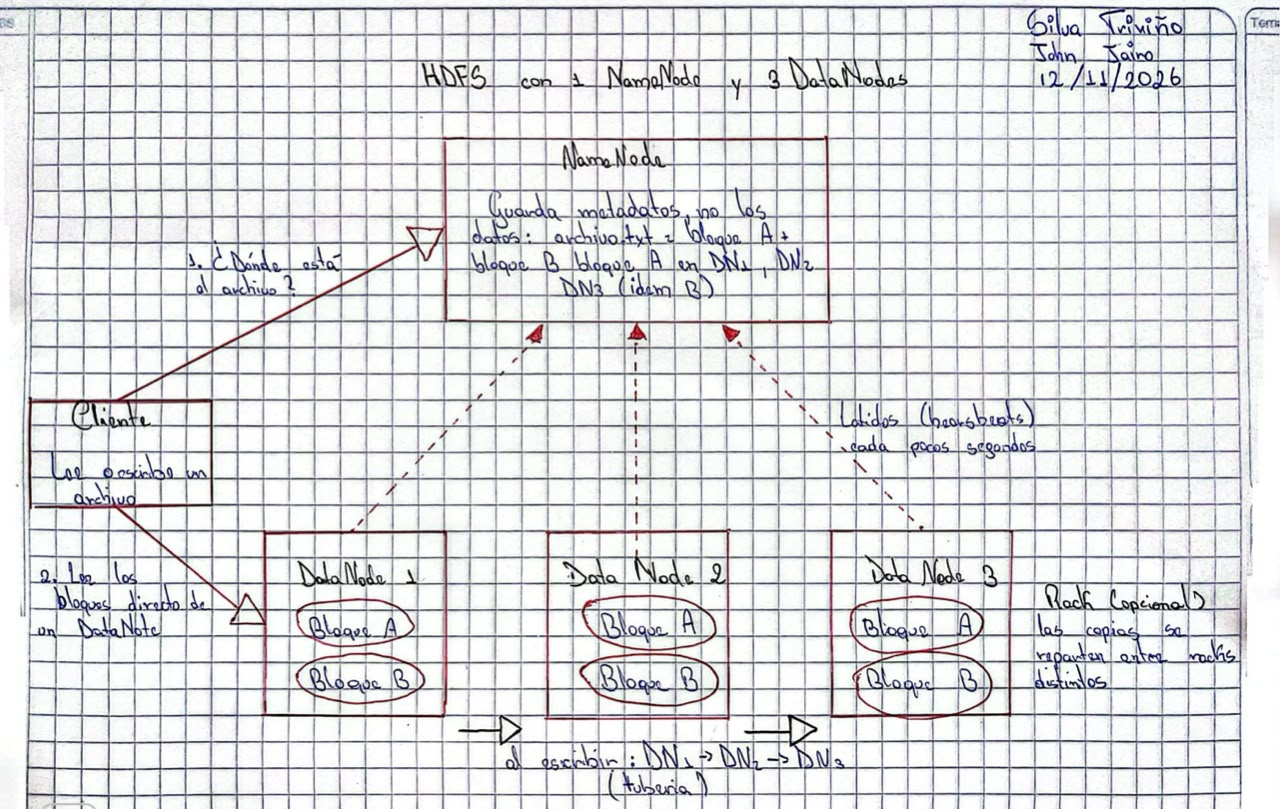
\includegraphics[width=\textwidth]{../figuras/Anexo-A-boceto-mano-HDFS.jpeg}
\caption{Boceto a mano de HDFS con 1 NameNode y 3 DataNodes (Silva Triviño John Jairo, 12/11/2026), punto de partida del diagrama de la figura~\ref{fig:arq}.}
\end{figure}

\section{Capturas de lectura de las fuentes}
Cada captura corresponde a una cita del informe; la página es la que se ve en el PDF.
\begin{figure}[H]
\centering
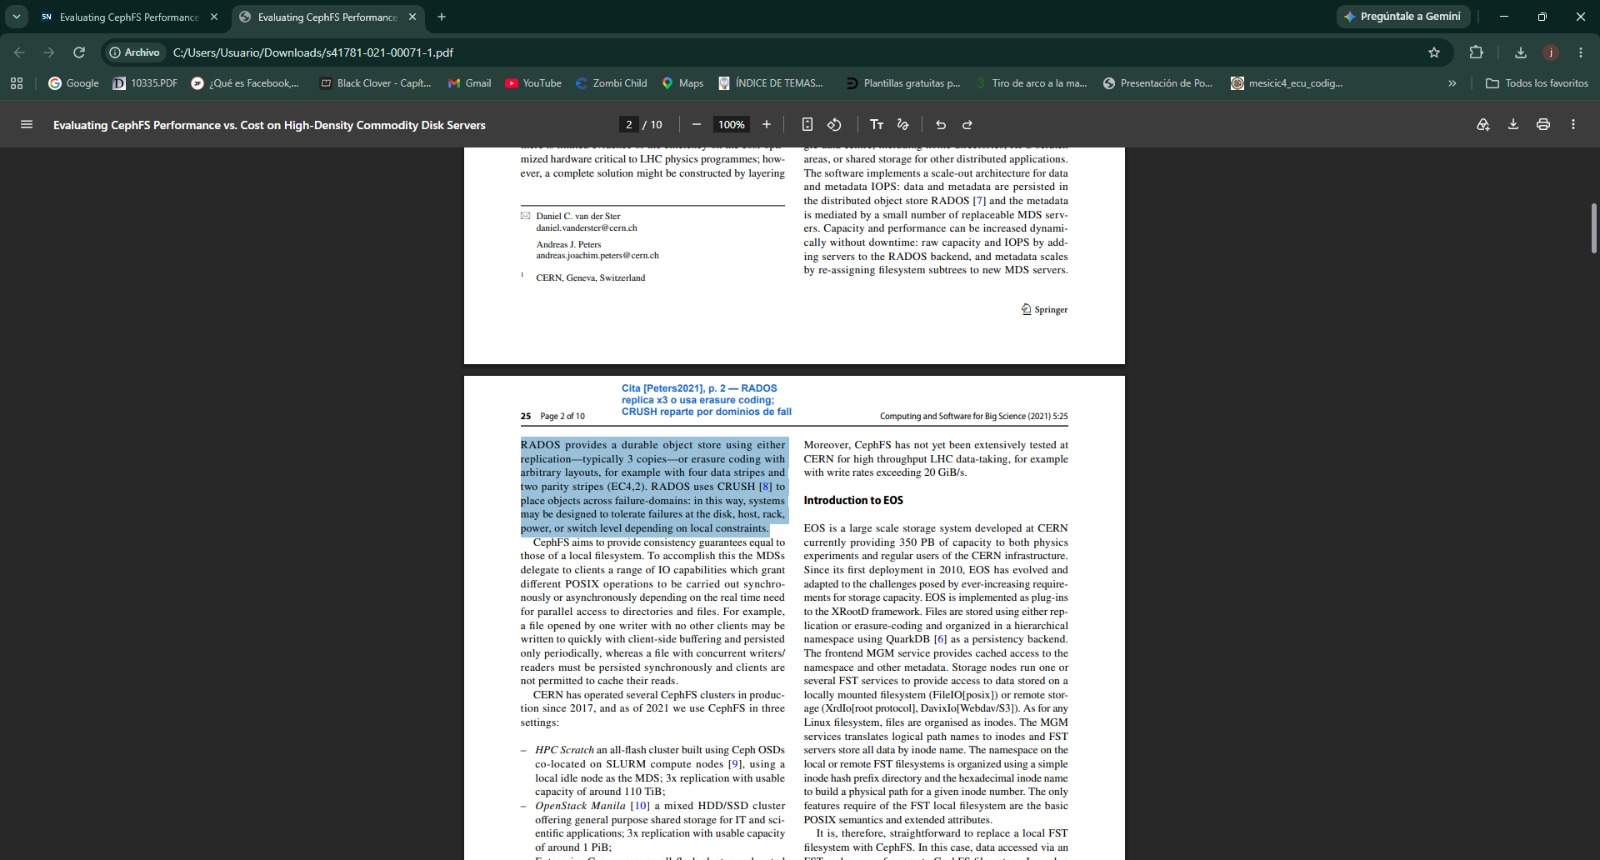
\includegraphics[width=\textwidth]{../capturas-lectura/lectura-01c-Peters2021-crush.jpeg}
\caption{Peters y van der Ster \cite{Peters2021}, p.~2: replicación o codificación por borrado, y CRUSH reparte por dominios de fallo.}
\end{figure}
\begin{figure}[H]
\centering
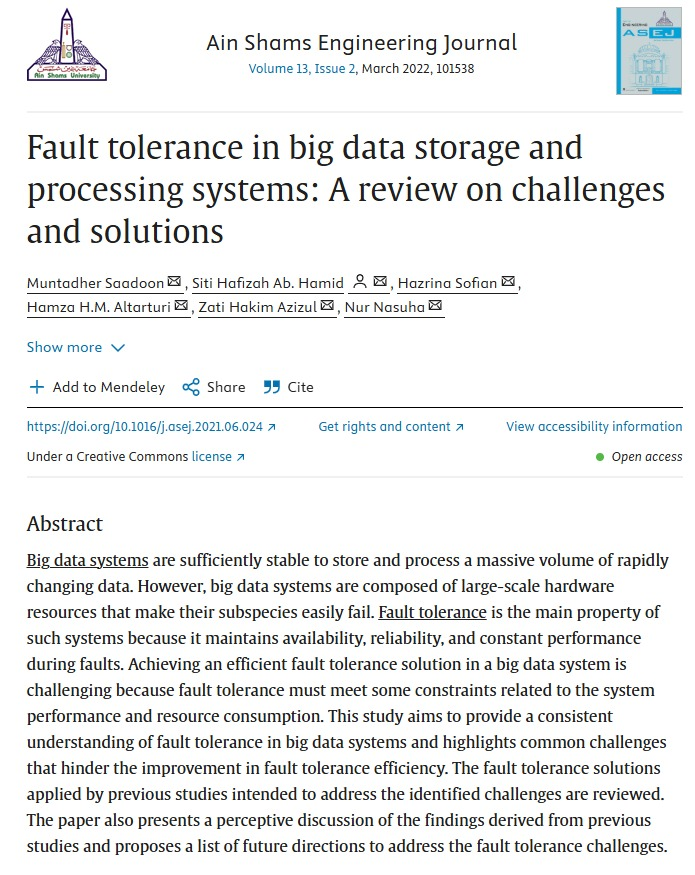
\includegraphics[width=\textwidth]{../capturas-lectura/lectura-02-Saadoon2022-heartbeat.jpeg}
\caption{Saadoon et al. \cite{Saadoon2022}, p.~3 del PDF: heartbeats y detección de fallos, usado en HDFS.}
\end{figure}
\begin{figure}[H]
\centering
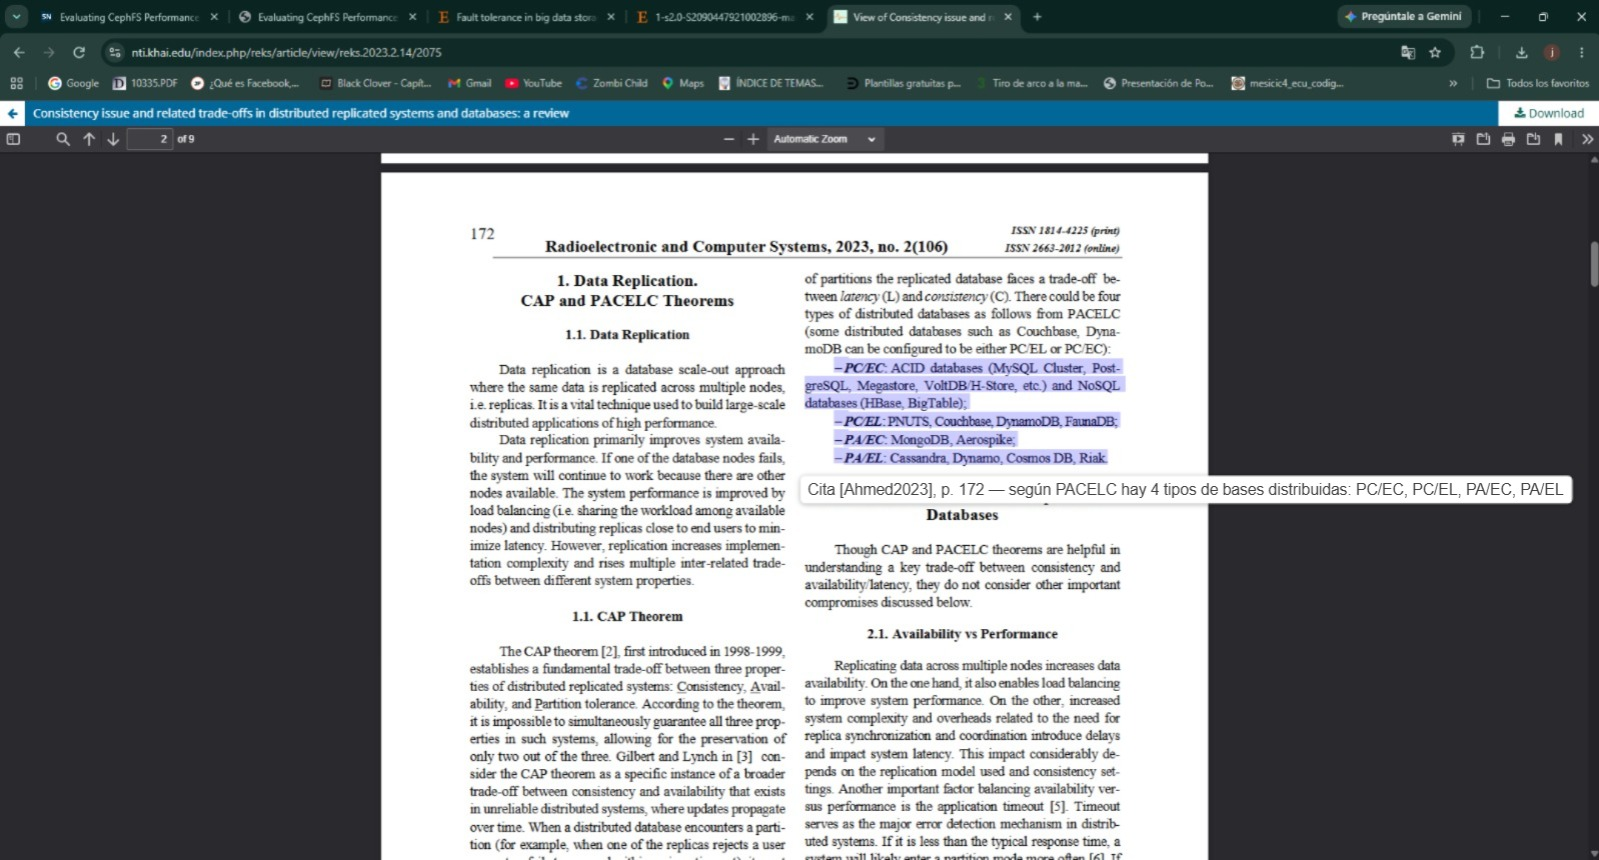
\includegraphics[width=\textwidth]{../capturas-lectura/lectura-03-Ahmed2023-pacelc.jpeg}
\caption{Ahmed et al. \cite{Ahmed2023}, p.~172: los cuatro tipos de PACELC.}
\end{figure}

\end{document}
